% fancytikzposter.tex, version 2.1
% Original template created by Elena Botoeva [botoeva@inf.unibz.it], June 2012
% 
% This file is distributed under the Creative Commons Attribution-NonCommercial 2.0
% Generic (CC BY-NC 2.0) license
% http://creativecommons.org/licenses/by-nc/2.0/ 


\documentclass{a0poster}

\usepackage{fancytikzposter} 


%%%%% --------- Change here if you want ---------- %%%%%
%% margin for the geometry package, must be changed before using the geometry package
%% default value is 4cm
% \setmargin{4}

%% the space between the blocks
%% default value is 2cm
% \setblockspacing{2}

%% the height of the title stripe in block nodes, decrease it to save space
%% default value is 3cm
% \setblocktitleheight{3}

%% the number of columns in the poster, possible values 2,3
%% default value is 2
% \setcolumnnumber{3}

%% the space between two or more groups of authors from different institutions
%% used in \maketitle
% \setinstituteshift{10}

%% which template to use
%% N1 simple, standard look, with a colored background and gray boxes
%% N2 board with nodes
%% N3 another standard look
%% N4 envelope-like look
%% N5 with a wave-like head, original idea taken from
%%%% http://fc09.deviantart.net/fs71/f/2010/322/1/1/scientific_poster_by_nabuy-d333ria.jpg
\usetemplate{5}

%% components of the templates
%% (the maximal possible numbers are mentioned as the parameters)
% \usecolortemplate{4}
% \usebackgroundtemplate{5}
% \usetitletemplate{2}
% \useblocknodetemplate{5}
% \useplainblocktemplate{4}
% \useinnerblocktemplate{2}


%% the height of the head drawing on top 
%% applicable to templates N3, 4 and 5
% \setheaddrawingheight{14}


%% change the basic colors
%\definecolor{myblue}{HTML}{008888} 
%\setfirstcolor{myblue}% default 116699
%\setsecondcolor{gray!80!}% default CCCCCC
%\setthirdcolor{red!80!black}% default 991111

%% change the more specific colors
% \setbackgrounddarkcolor{colorone!70!black}
% \setbackgroundlightcolor{colorone!70!}
% \settitletextcolor{textcolor}
% \settitlefillcolor{white}
% \settitledrawcolor{colortwo}
% \setblocktextcolor{textcolor}
% \setblockfillcolor{white}
% \setblocktitletextcolor{colorone}
% \setblocktitlefillcolor{colortwo} %the color of the border
% \setplainblocktextcolor{textcolor}
% \setplainblockfillcolor{colorthree!40!}
% \setplainblocktitletextcolor{textcolor}
% \setplainblocktitlefillcolor{colorthree!60!}
% \setinnerblocktextcolor{textcolor}
% \setinnerblockfillcolor{white}
% \setinnerblocktitletextcolor{white}
% \setinnerblocktitlefillcolor{colorthree}




%%% size of the document and the margins
%% A0
% \usepackage[margin=\margin cm, paperwidth=118.9cm, paperheight=84.1cm]{geometry} 
\usepackage[margin=\margin cm, paperwidth=84.1cm, paperheight=118.9cm]{geometry}
%% B1
% \usepackage[margin=\margin cm, paperwidth=70cm, paperheight=100cm]{geometry}



%% changing the fonts
\usepackage{cmbright}
%\usepackage[default]{cantarell}
%\usepackage{avant}
%\usepackage[math]{iwona}
\usepackage[math]{kurier}
\usepackage[T1]{fontenc}
\usepackage{subfig}
\usepackage{graphicx}
\usepackage{float}
%% add your packages here
\usepackage{hyperref}

\def\Put(#1,#2)#3{\leavevmode\makebox(0,0){\put(#1,#2){#3}}}



\title{SIFT descriptor to set landmark on biological images}
\author{Van Linh LE$^{1,3}$, Marie BEURTON-AIMAR$^1$, Adrien KRAHENBUHL$^1$, Nicolas PARISEY$^2$\\
  $^1$LaBRI - UMR 5800, Univ. Bordeaux, $^2$INRA - IGEPP UMR 1349, France $^3$ IT - DLU,Vietnam\\
  \texttt{van-linh.le,beurton,adrien.krahenbuhl@labri.fr,nparisey@rennes.inra.fr}
}


\begin{document}

%%%%% ---------- the background picture ---------- %%%%%
%% to change it modify the macro \BackgroundPicture
\ClearShipoutPicture
\AddToShipoutPicture{\BackgroundPicture}

\noindent % to have the picture right in the center
\begin{tikzpicture}
  \initializesizeandshifts
  % \setxshift{15}
  % \setyshift{2}


  %% the title block, #1 - shift, the default value is (0,0), #2 - width, #3 - scale
  %% the alias of the title block is `title', so we can refer to its boundaries later
  \ifthenelse{\equal{\template}{1}}{ 
    \titleblock{47}{1}
  }{
    \titleblock{47}{1.4}
  }

  %% a logo can be added to the title block
  %% #1 - anchor relative to the title block, #2 - shift, #3 - width, #3 - file name
  % \ifthenelse{\equal{\template}{2}}{ 
  %   \addlogo[south west]{(2,0)}{6cm}{unibz_b.png}
  % }{
  %   \addlogo[south west]{(2,0)}{6cm}{unibz_w.png}
  % }


  %% a block node, with the specified position (optional), title and the content
  %% #1 - where (optional), #2 - title, #3 - text
  %%%%%%%%%% ------------------------------------------ %%%%%%%%%%
  \blocknode%
  {Context}%
  {
	  \begin{itemize}
   		 \item Morphometry analysis is a way to characterize the shape variations of the organisms,
   		 \item Morphometric characteristics have been used to evaluate the evolution of an organism or classification.
   		 \item ...
    	  \end{itemize}
%    	  \begin{tikzfigure}
%    	  	\centering
%    	  	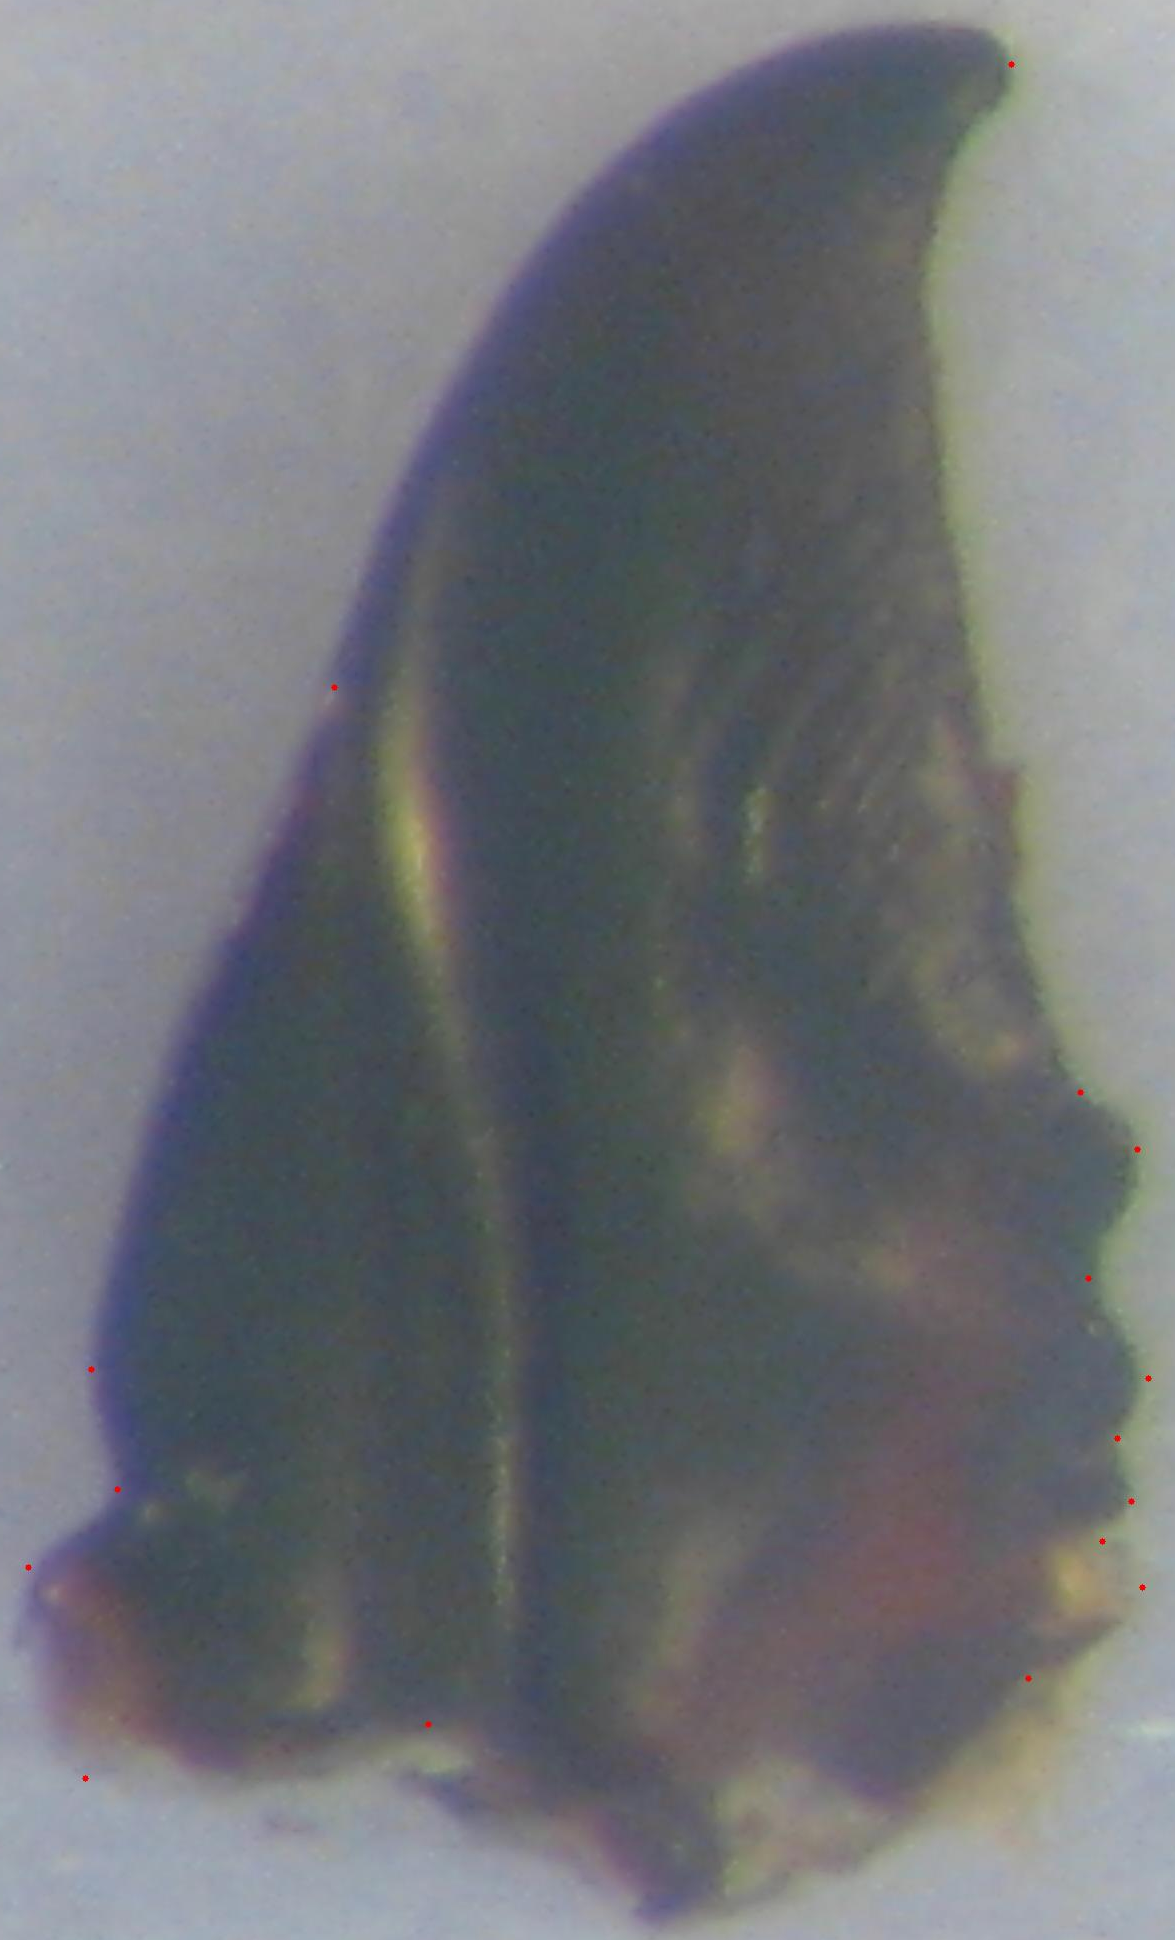
\includegraphics[width=0.3\textwidth]{images/color}~~~~~~
%    	  	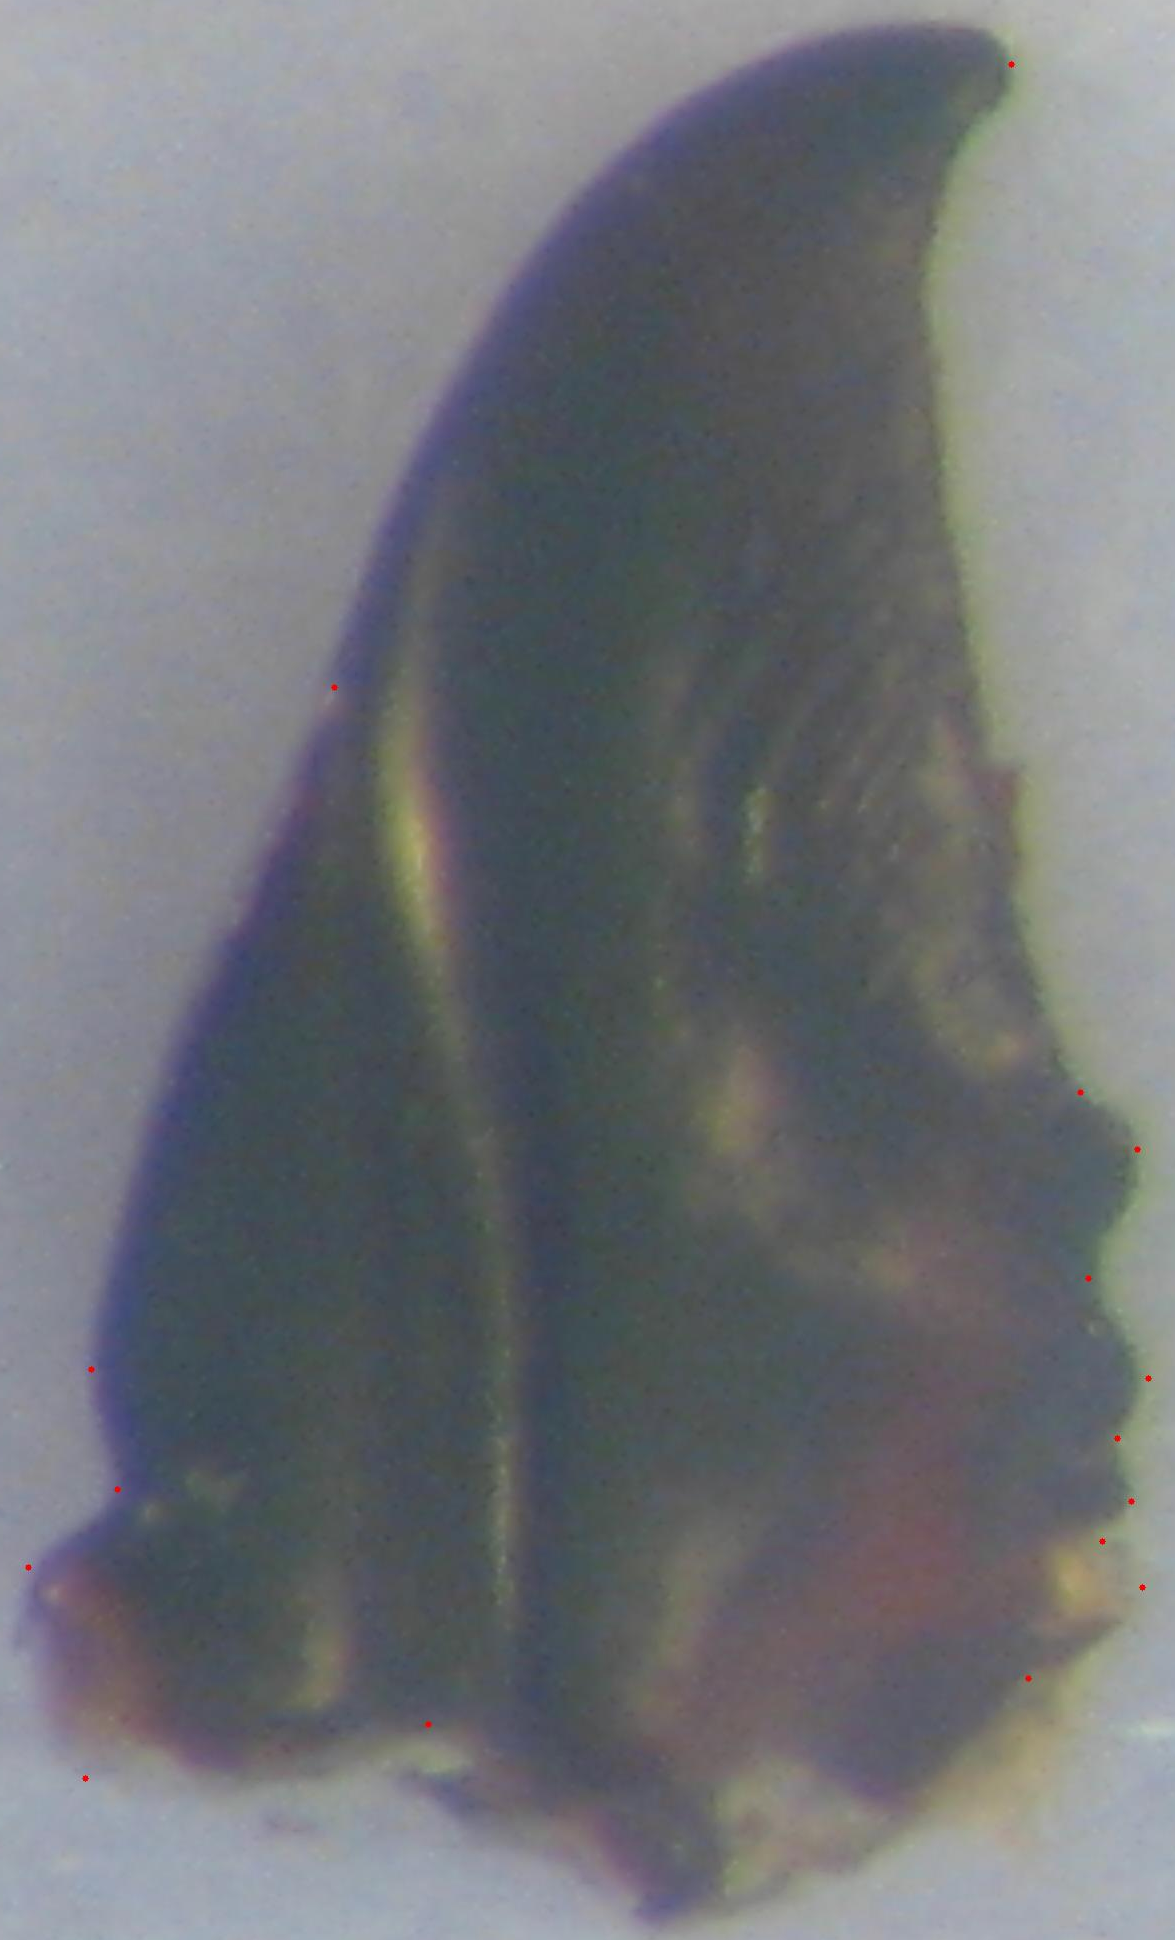
\includegraphics[width=0.3\textwidth]{images/color}
%    	  \end{tikzfigure}
    	  
  }


  %% a callout block
  %% #1 - rotate angle (optional), #2 - from, #3 - where, #4 - width, #5 - text
  %%%%%%%%%% ------------------------------------------ %%%%%%%%%%
  %\calloutblock{($(box.center)+(-2,-8)$)}
  %{($(box.center)+(10,-1)$)}
  %{19cm}
  %{\small
  %  Macro for creating a block node:
  %  \begin{itemize}
  %  \item[] \textbackslash blocknode\{Block Title\}\{Block Content\}
  %  \end{itemize}
  %  Macro \textbackslash blocknode has three parameters. The first one is
  %  optional and it is the position of the block. The first block will be
  %  automatically placed to (\$(firstrow)-(xshift)-(yshift)\$), which is the
  %  left corner below the title block. In most of the templates, (firstrow) is
  %  set to (title.south), where \emph{title} is the alias for the title
  %  block. Each subsequent block is automatically placed to
  %  [(\$(box.south)-(yshift)\$)], i.e., below the previous block aliased
  %  \emph{box}.  You can also use an explicit parameter, e.g., $(-10,30)$ (note
  %  that (0,0) is the center of the poster). The second parameter is the title
  %  of the block. Finally, the last parameter is the  actual content. 
  %}




  %% by default, the position of the new block node is right below the previous
  %% block node, stored in (currenty)
  %% box is the alias of the previous block, so we can refer to its boundaries

  %%%%%%%%%% ------------------------------------------ %%%%%%%%%%
  \blocknode{Manual landmarks}%
  {
  	\begin{itemize}
  		\item Morphometric landmarks are points that are a kind of points of interest,
  		\item Landmarks are along an image outline and contain a lot of important information,
  		\item They are defined by the biologists. 
  	\end{itemize}
  	\begin{tikzfigure}[The mandibles with manual landmarks]
    	  	\centering
    	  	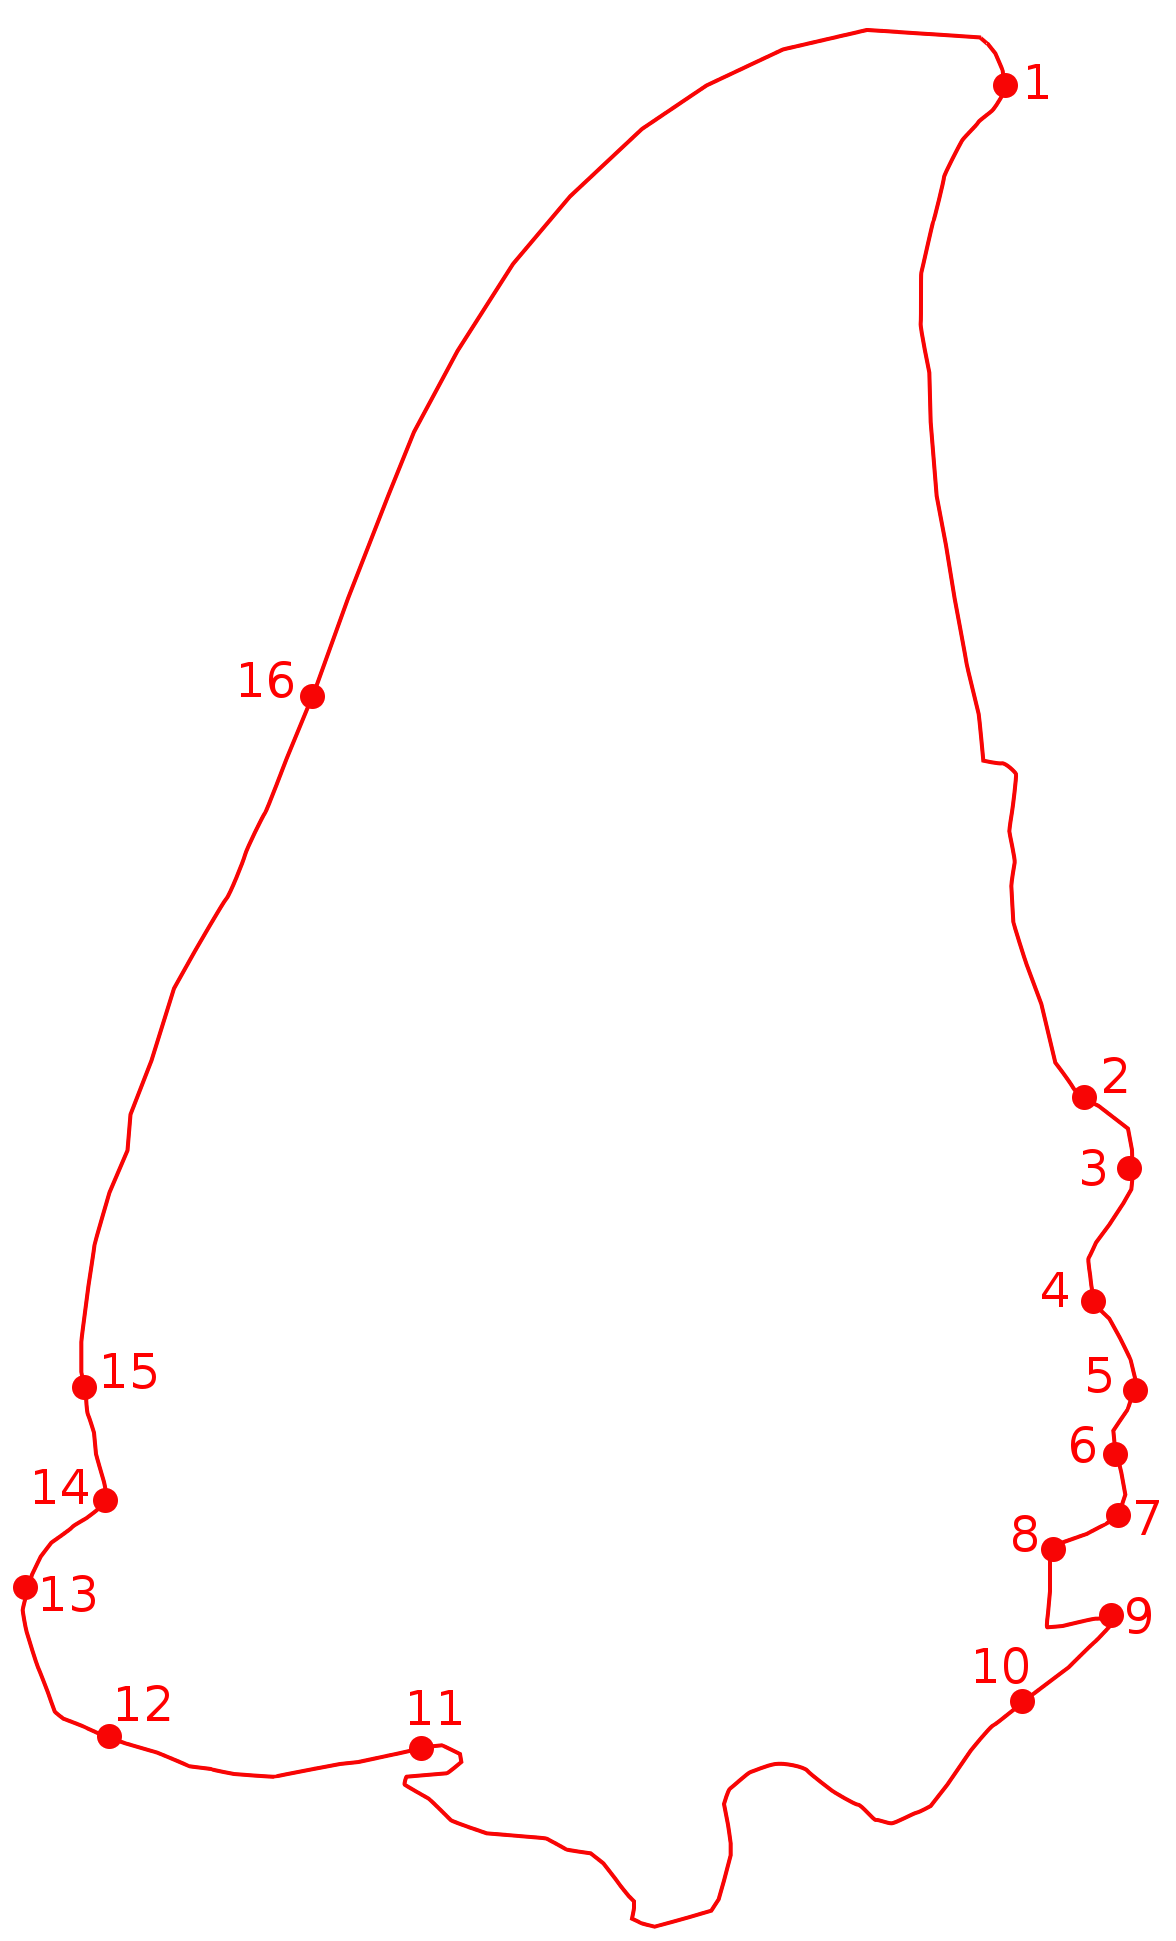
\includegraphics[width=0.3\textwidth]{images/mlandmarksline}~~~~~~
    	  	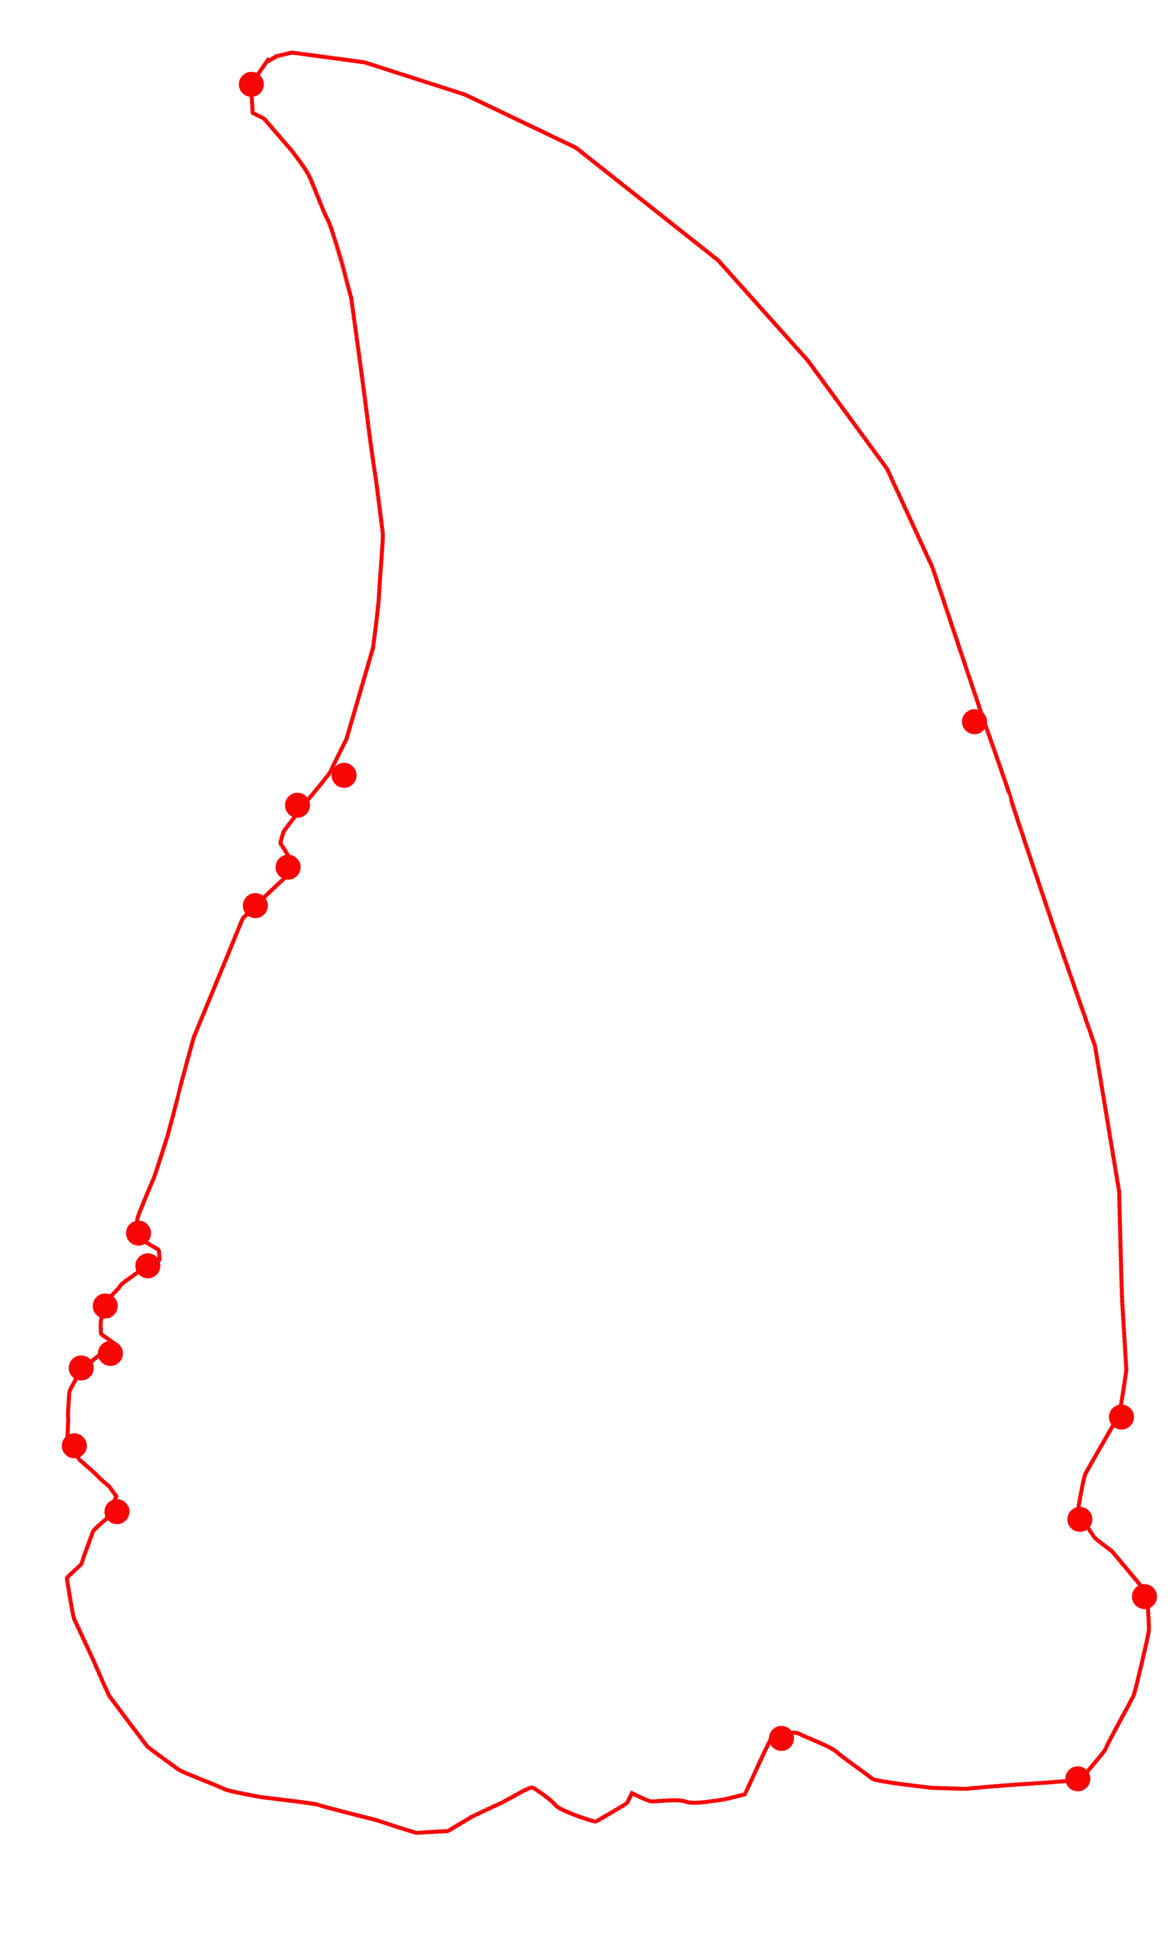
\includegraphics[width=0.3\textwidth]{images/mglandmarksline}
    	  \end{tikzfigure}
    	How to locate the landmarks automatically?
  }
  

  %%%%%%%%%% ------------------------------------------ %%%%%%%%%%
  \blocknodew[($(currenty)-(3.5,0)$)]{30}{SIFT and landmarks} %
  { SIFT\cite{•} is used to extract distinctive features from the images. 
  It includes four steps:
    \begin{itemize}
    		\item Scale-space extrema detection
    		\item Keypoints localization
    		\item Orientation assigment
    		\item Keypoint descriptor
    \end{itemize}~\\
    \Put(18,7){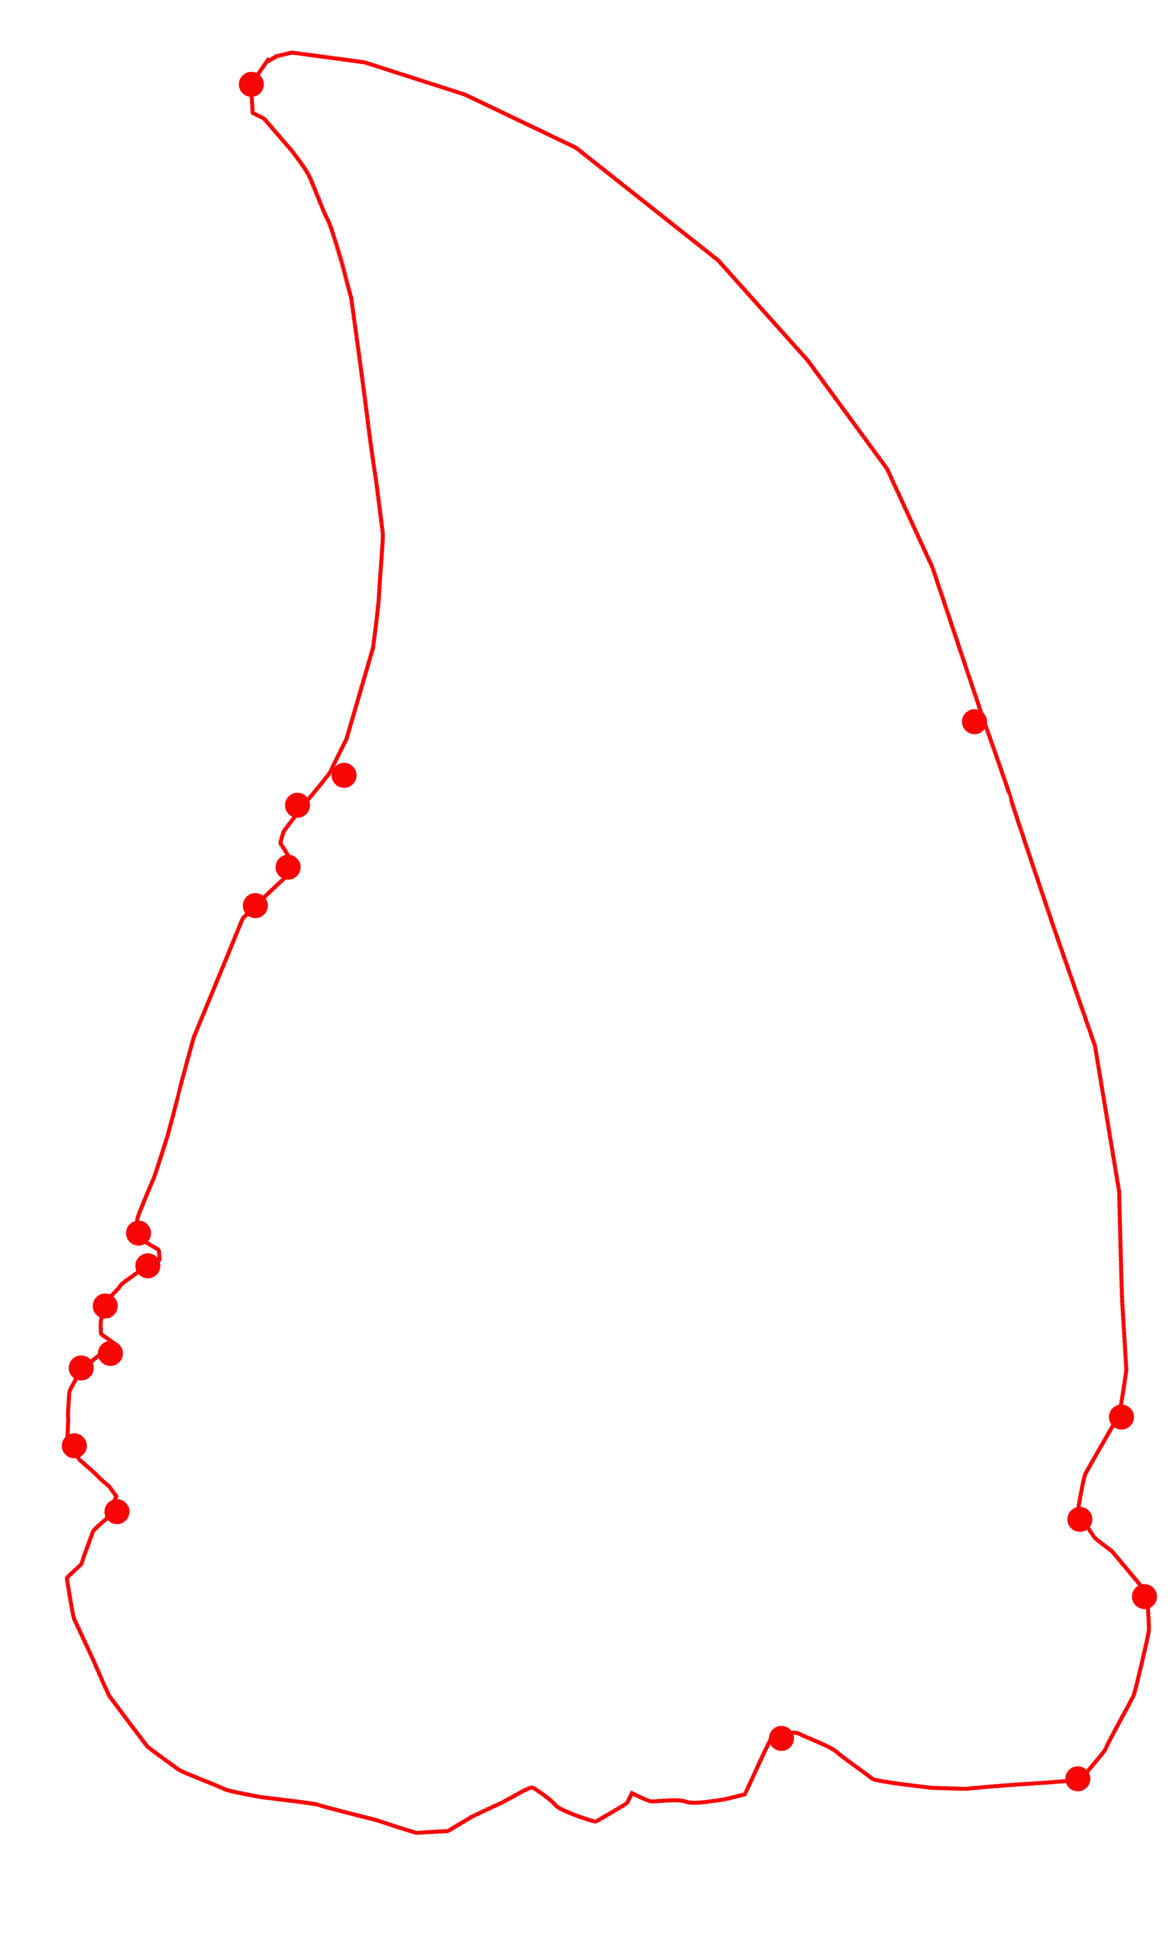
\includegraphics[scale=0.2]{images/mglandmarksline}}
    The original SIFT outputs many candidates \\
    for landmarks.\\
    \textbf{\underline{Solution:}} Limiting the searching space before computing\\
    the SIFT descriptors.  
  }
 
 %%%%%%%%%%%%%%%%%%%%%%%%%%%%%%%%%%%%%%%%%%%%%%%%%%%%%%%%%%%%%%%%%%%%%%%%%%
  \blocknode[($(currenty)+(3.5,0)$)]{Proposed method}
  {
  	\begin{tikzfigure}
    	  	\centering
    	  	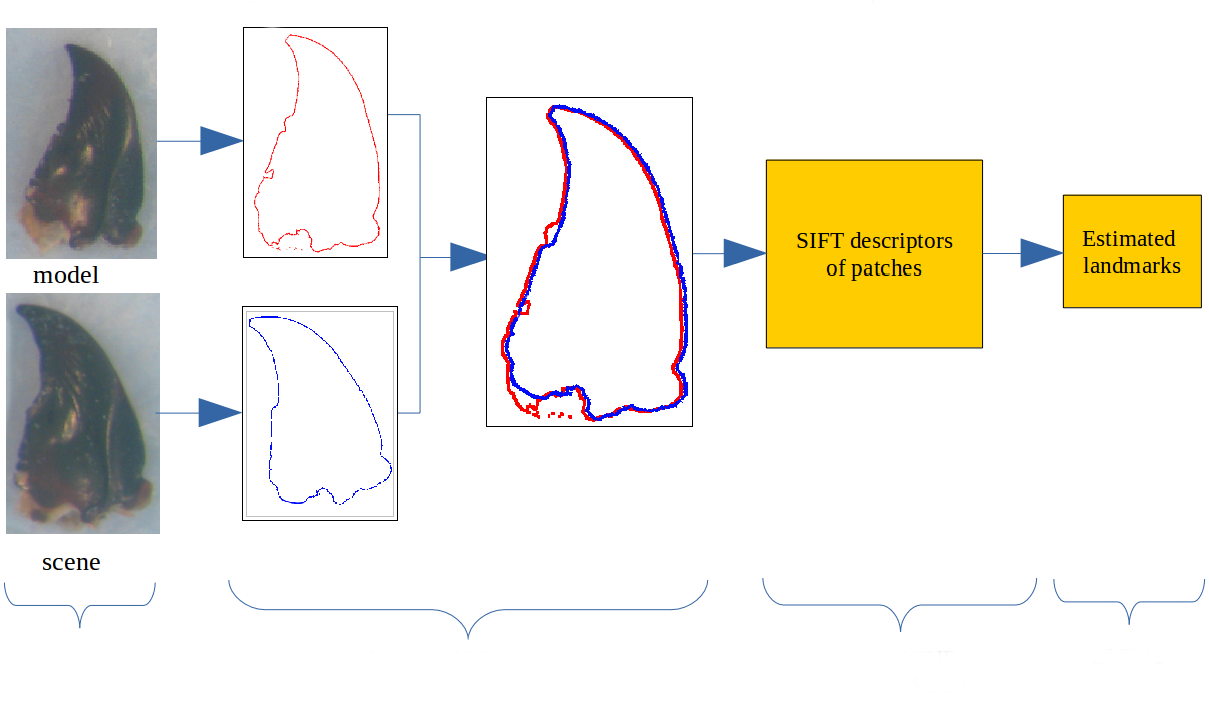
\includegraphics[width=0.9\textwidth]{images/method2}
    	  \end{tikzfigure}
  }
  
  
  %\useplainblocktemplate{3}
  %\plainblock[0]{($(currenty)+(2,0)$)}{35}{} %
  %{
    
  %  abc
  %  }
 
  %%%%%%%%%%%%% NEW COLUMN %%%%%%%%%%%%%%% 
  \startsecondcolumn 

  %%%%%%%%%% ------------------------------------------ %%%%%%%%%%
  \blocknode%
  {Segmentation}%
  {
    \begin{itemize}
		\item Converting the image to binary by applying binary threshold. 
		The threshold value is determined by analysing histogram\cite{•}.
		\item Contours points are extracted by Canny algorithm\cite{•}.
		\item The threshold ratio in Canny: $T_{lower} = (1/3) \times T_{upper}$
    \end{itemize}
  }


  
  %%%%%%%%%% ------------------------------------------ %%%%%%%%%%
  \blocknode{Registration}%
  {There are three types of colored boxes/blocks that you can use inside block
    nodes to highlight information. \\
    
    \begin{tabular}[t]{ll}
      \begin{minipage}{0.5\linewidth}
        \innerblock{Theorem} {Statement}
      \end{minipage}
      & 
      \textbackslash innerblock\{Theorem\}\{Statement\}\\

      \begin{minipage}{0.5\linewidth}
        \innerblockplain[colorone!80!]{Text}
      \end{minipage}
      &
      \textbackslash innerblockplain[colorone!80!]\{Text\}\\ 

      \begin{minipage}{0.5\linewidth}
        \coloredbox{colorthree!50!}{Text}
      \end{minipage}
      &
      \textbackslash coloredbox\{colorthree!50!\}\{Text\}
    \end{tabular}

    \vspace{0.5cm}
    The default figure environment does not work within a tikzpicture. I created
    a new figure environment that can be used instead, based on the code sent by
    Stephan Thober.
    \begin{itemize}
    \item[] \textbackslash begin\{tikzfigure\}[Caption]\\
      \ldots\\
      \textbackslash end\{tikzfigure\}
    \end{itemize} 
    % 

    \begin{tikzfigure}[A shaded circle]
      \begin{tikzpicture}
        \draw[draw=none,inner color=colorthree, outer color=colorone] (0,0) circle (2cm);
      \end{tikzpicture}
    \end{tikzfigure}
  }


  %%%%%%%%%% ------------------------------------------ %%%%%%%%%%
  %\calloutblock{($(box.south east)-(8,-2)$)}
  %{($(box.south east)-(16,2)$)}
  %{30cm}
  %{
  % There are also callout blocks that allow for a more interesting layout of the poster. 
  %  \begin{itemize}
  %  \item[] \textbackslash calloutblock[rotate angle]\{from
  %    coordinate\}\{coordinate\}\{Block Width\}\{Block Content\} 
  %  \end{itemize}
  %  The alias for such blocks is \emph{note}.
  %}


  %% to place the next node centered vertically in the second column, we can
  %% obtain the y-coordinate of the previous node using macro
  %% \getcurrentrow{note}, where note is the alias of the callout node, and
  %% then specify the coordinate of the next node using coordinate (currentrow)
  %\getcurrentrow{note}


  %% a plain block
  %% #1 - rotate angle (optional), #2 - where, #3 - width, #4 - title, #5 - text
  %%%%%%%%%% ------------------------------------------ %%%%%%%%%%
  %\plainblock{($(currentrow)+(xshift)-(yshift)$)}%[($(currenty)+(0,10)$)]%
  %{32}{Plain blocks} %
  %{These blocks are similar to callout blocks. They allow for specifying the
  %  title of the block.
  %  \begin{itemize}
  %  \item[] \textbackslash plainblock[rotate angle]\{coordinate\}\{Block Width\}\{Block
   %   Title\}\{Block Content\} 
   % \end{itemize}
  %}


 
  %% the coordinate (currenty) is used in the default placing of the next blocknode
 %\getcurrentrow{note}
 %\coordinate (currenty) at ($(currentrow)+(xshift)-(yshift)$);



   %%%%%%%%%%%%% NEW COLUMN %%%%%%%%%%%%%%% 
  %% (if column number is 3)
 % \startthirdcolumn

  %%%%%%%%%% ------------------------------------------ %%%%%%%%%%
  \blocknode {Result}
  {It is possible to adjust the layout of the poster. To impose your own
    setting, you can use these macros:
    \begin{itemize}
    \item Macros for changing sizes
      \begin{itemize}
      \item[] \textbackslash setmargin\{4\},
        %% the height of the head drawing on top
        %% applicable to templates N2 and 4
        \textbackslash setheaddrawingheight\{14\},
        %% the space between two or more groups of authors from different
        %% institutions
        %% used in \maketitle
        \textbackslash setinstituteshift\{10\},\\
        %% the space between the blocks
        %% default value is 2cm
        \textbackslash setblockspacing\{2\},
        %% the height of the title stripe in block nodes, decrease it to save space
        %% default value is 3cm
        \textbackslash setblocktitleheight\{3\}
      \end{itemize}

    \item Other structural macros
      \begin{itemize}
      \item[]  %% the number of columns in the poster, possible values 2,3
        %% default value is 2
        \textbackslash setcolumnnumber\{3\},
        %% which template to use 
        %% N1 simple, standard look, with a colored background and gray boxes
        %% N2 board with nodes
        %% N3 another standard look
        %% N4 envelope like look
        %% N5 with a wave-like head, original idea taken from
        %%%% http://fc09.deviantart.net/fs71/f/2010/322/1/1/scientific_poster_by_nabuy-d333ria.jpg
        %% N6 experimental, oriental style, largely based on template N3
        \textbackslash usetemplate\{6\},\\
        \textbackslash usecolortemplate\{4\},
        \textbackslash usebackgroundtemplate\{5\},
        \textbackslash usetitletemplate\{2\},\\
        \textbackslash useblocknodetemplate\{5\},
        \textbackslash useinnerblocktemplate\{3\},
        \textbackslash useplainblocktemplate\{4\}

      \end{itemize}

    \item Macro for adding logos to the title block
      \begin{itemize}
      \item[] \textbackslash addlogo[south west]\{(0,0)\}\{6cm\}\{filename\}
      \end{itemize}

    \item Macros for the basic colors
      \begin{itemize}
      \item[] \textbackslash setfirstcolor\{green!70!\}, % default 116699
        \textbackslash setsecondcolor\{gray!80!\}, % default CCCCCC
        \textbackslash setthirdcolor\{red!80!black\}% default 991111
      \end{itemize}

    \item Macros for specific colors:
      \begin{itemize}
      \item[] \textbackslash setbackgrounddarkcolor\{colorone!70!black\},
        \textbackslash setbackgroundlightcolor\{{\small colorone!70!}\},\\
        \textbackslash settitletextcolor\{textcolor\},
        \textbackslash settitlefillcolor\{white\},
        \textbackslash settitledrawcolor\{colortwo\},\\
        \textbackslash setblocktextcolor\{textcolor\},
        \textbackslash setblockfillcolor\{white\},\\
        \textbackslash setblocktitletextcolor\{colorone\},
        \textbackslash setblocktitlefillcolor\{colortwo\}, \\
        \textbackslash setplainblocktextcolor\{textcolor\},
        \textbackslash setplainblockfillcolor\{colorthree!40\},\\
        \textbackslash setplainblocktitletextcolor\{textcolor\},
        \textbackslash setplainblocktitlefillcolor\{colorthree!60\}, \\
        \textbackslash setinnerblocktextcolor\{textcolor\},
        \textbackslash setinnerblockfillcolor\{white\},\\
        \textbackslash setinnerblocktitletextcolor\{white\},
        \textbackslash setinnerblocktitlefillcolor\{colorthree\},
      \end{itemize}
    \end{itemize}
  }

%%%%%%%%%% ------------------------------------------ %%%%%%%%%%
  \blocknode%
  {Bibliography}%
  {To start the second column or the third column use commands
    \begin{itemize}
    \item[] \textbackslash startsecondcolumn, and \textbackslash startthirdcolumn.
    \end{itemize}
    If the number of columns is 2, then the last command will not have
    effect. \\

    You can also start a new column with an arbitrary x-coordinate by specifying
    explicitly the coordinate of the new block node as follows:
    \begin{itemize}
    \item[] \textbackslash blocknode[(\$(firstrow)-(yshift)+(x,0)\$)]\{Block
      Title\}\{Block Content\}
    \end{itemize}

    % 
  }


\end{tikzpicture}


\end{document}




